\chapter{Appendix: Resonator Fitting\label{ch:AppA}}

A large part of the experimental work done in this thesis involves probing 3D cavity resonators using classical microwave fields. In doing so, we are able to infer various properties of the resonator such as its internal and coupling losses. In this appendix, we derive from first principles the resonance lineshape of a single-mode resonator coupled a readout transmission line. This simple example can be treated theoretically using the \textit{input-output formalism}, yet it is general enough to cover several of the experiments performed in this thesis. In order to bridge the gap between this model and our experimental setup, we also extend our analysis to the include (a) reflection measurements using a circulator, (b) asymmetric lineshapes due to so-called Fano resonances, and (c) the calculation of transmission coefficients when the mode is connected to separate transmission lines. 

\section{Input-Output Theory for Resonators}
\subsection{Single-Mode Reflection Measurements}

Let's consider a linear resonator mode $\hat{a}$ with angular frequency $\omega_0$ coupled to a transmission line. The Hamiltonian describing this mode is that of a quantum harmonic oscillator, $\hat{H} = \myhbar\omega_0 \hat{a}^\dagger \hat{a}$. Without the transmission line, the dynamics of $\hat{a}$ are given in the Heisenberg picture by $\partial_t\hat{a} = -i[\hat{a}, \hat{H}] = -i\omega_0\hat{a}$, which leads to the familiar oscillatory motion of $\hat{a}(t)$ in phase space. However, if we include losses and coupling to the transmission line, the dynamics are modified in the form of a Heisenberg-Langevin equation \cite{walls1994quantum, gardiner2004quantum, clerk2010introduction}:
\begin{equation}
    \odv*{\hat{a}}{t}(t) = -i\omega_0\hat{a} - \Big(\frac{\kappa_c + \kappa_i}{2}\Big)\hat{a} + \sqrt{\kappa_c}\hat{a}_{\rm in}(t)
    \label{eq:A_heisenberg}
\end{equation}
Here, we include a damping term proportional to the total loss rate $\kappa = \kappa_c + \kappa_i$, where $\kappa_i$ is the \textit{intrinsic loss} of the mode due to uncontrolled interaction with environmental degrees of freedom and $\kappa_c$ is the \textit{coupling loss} to the transmission line (which we as experimenters may control for in design)\footnote{For a full derivation of this Heisenberg-Langevin equation in the context of superconducting circuits, two great expository references are the PhD theses of Audrey Bienfait \cite{bienfait2016thesis} and Steven Touzard \cite{touzard2019thesis}.}. The propagating fields inside  the transmission line are given by $\hat{a}_{\rm out}$ and $\hat{a}_{\rm in}$, as shown in Fig. \ref{fig:A_InputOutput}, with the latter giving rise to the source term $\sqrt{\kappa_c}\hat{a}_{\rm in}(t)$ in Eq. \eqref{eq:A_heisenberg}. At this point, let's also stop to introduce some useful terminology. If $\kappa_i < \kappa_c$, we refer to the resonator as \textit{overcoupled} and if $\kappa_i > \kappa_c$, we call it \textit{undercoupled}. Finally, if $\kappa_i = \kappa_c$, then the resonator is called \textit{critically coupled}. We will elaborate on the distinction between these cases later in this section. 


\begin{figure}[h]
    \centering
    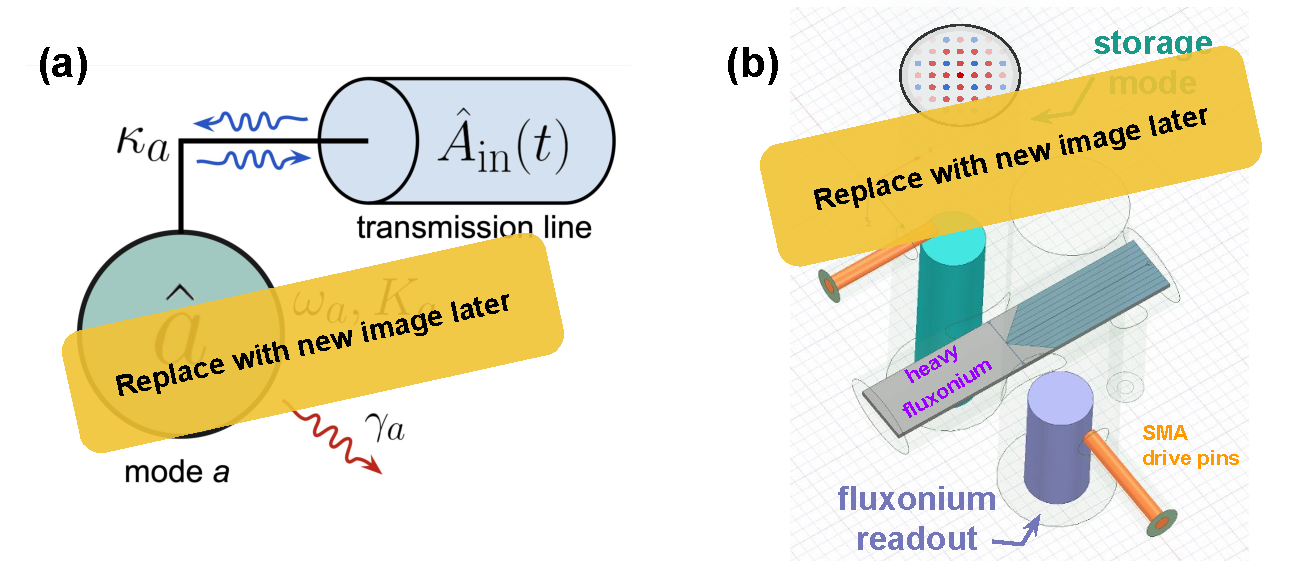
\includegraphics[width=0.8\linewidth]{Figures/A/InputOutput.pdf}
    \caption{\textbf{(a)} Resonator mode $\hat{a}$ coupled to a transmission line is modeled via Eq. \eqref{eq:A_heisenberg}. \textbf{(b)} This setup can be realized using the electric field of a 3D superconducting post cavity.}
    \label{fig:A_InputOutput}
\end{figure}

\noindent In circuit QED experiments, we typically interact with readout resonators using a classical field $\alpha_{\rm in}(t)$ associated with a coherent state $\ket{\alpha_{\rm in}}$ in the input transmission line. Taking the expectation value on both sides of Eq. \eqref{eq:A_heisenberg}, we get $\partial_t \hat{a}(t) = -i\omega_0\hat{a} - (\kappa_c + \kappa_i)\hat{a}/2 + \sqrt{\kappa_c}\alpha_{\rm in}(t)$. Note that by defining the drive amplitude $\epsilon(t) = i\sqrt{\kappa_c}\alpha_{\rm in}(t)$, we can now self-consistently interpret the source term as coming from a Hamiltonian drive $\epsilon(t)(\hat{a} + \hat{a}^\dagger)$ on the system. 

If we examine the mean-value intra-resonator field $\alpha(t) = \ev{\hat{a}}(t)$ and take the Fourier transform $\mathcal{F}[\bullet]$ on both sides of the resulting equation, we can calculate\footnote{Recalling the definition $\mathcal{F}[\alpha(t)] \equiv \int \alpha(t) e^{i\omega t}dt$, we can derive $\mathcal{F}[\partial_t\alpha(t)] = -i\omega \alpha(\omega)$ via integration by parts.} the frequency domain response:
\begin{equation}
    \alpha(\omega) = \frac{2\sqrt{\kappa_c}}{\kappa_c + \kappa_i - 2i(\omega-\omega_0)} \alpha_{\rm in}(\omega)
    \label{eq:inputoutput-freq-domain}
\end{equation}
This equation gives us the ability to calibrate the mean circulating photon number $\bar{n} = |\alpha|^2$ in the resonator, in terms of the input power $P_{\rm in} = \myhbar\omega |\alpha_{\rm in}|^2$ seen by the device. Specifically, on resonance ($\omega = \omega_0$), we get:
\begin{equation}
    \bar{n} = \frac{4\kappa_c P_{\rm in}}{\myhbar\omega_0(\kappa_c + \kappa_i)^2}
\end{equation}
For overcoupled readout resonators with $\kappa_i \ll \kappa_c$, this reduces to $P_{\rm in} = \kappa_c\myhbar\omega_0 \bar{n}/4$. 

\noindent Now, the classical continuity equation for the propagating fields gives rise to the so-called \textit{input-output relation} \cite{clerk2010introduction}, which expresses the resonator mode $\hat{a}$ in terms of the transmission line fields: 
\begin{equation}
    \hat{a}_{\rm in}(t) + \hat{a}_{\rm out}(t) = \sqrt{\kappa_c} \hat{a}(t)
    \label{eq:inputoutput}
\end{equation}
In combination with Eq. \eqref{eq:inputoutput-freq-domain}, this relation allows us to express the reflected coherent output signal $\alpha_{\rm out}(\omega)$ in terms of the input signal $\alpha_{\rm in}(\omega)$ sent in to the resonator. In particular, their ratio defines
\begin{equation}
   S_{11}(\omega) = \frac{\alpha_{\rm out}(\omega)}{\alpha_{\rm in}(\omega)} = \frac{\kappa_c - \kappa_i + 2i(\omega - \omega_0)}{\kappa_c + \kappa_i - 2i(\omega - \omega_0)},
\end{equation}
i.e. a reflection coefficient. The choice to call this coefficient $S_{11}$ can be traced back to the S-matrix formalism \cite{kurokawa1965power, gardiner1985input}, which extends the analysis here to multi-port devices, and defines $S_{ij}(\omega) = \alpha_{{\rm out}, i}(\omega)/\alpha_{{\rm in}, j}(\omega)$. In this case, we only have a single-port resonator, and the reflected signal is given by $S_{11}(\omega)$; this is also what we measure experimentally using a Vector Network Analyzer (VNA). 

\section{Experimental Considerations}

\subsection{Fitting the Background}
Low order polynomial fits etc.

\subsection{Fano Resonance: Asymmetry in the Lineshape}
Modify the fit function to 